\documentclass{article}

% Font
\usepackage[T1]{fontenc}
\usepackage[utf8]{inputenc}
\usepackage{lmodern}

% For symbols
\usepackage{pifont}
\newcommand{\xmark}{\ding{53}} % x

% For tables
\usepackage{adjustbox}
\usepackage{multirow}
\usepackage{color, colortbl}
\definecolor{Gray}{gray}{0.95}
\usepackage{hhline}

% For identing the table at the right place
\usepackage{float}

% For left spacing
\usepackage{scrextend}

% For images
\usepackage{graphicx}
\graphicspath{ {./images/} }

% links
\usepackage{hyperref}

% for shorter paragraph spaces
\setlength{\parindent}{1ex}
\setlength{\parskip}{0.5ex}
% for first paragraphs
\newcommand*\fpar{\hspace{1ex}}

\title{Project - Phase 8 Report}
\author{Group 14 \\
Tiago Carvalho fc51034 \\
Diogo Lopes fc51058 \\
Miguel Saldanha fc51072 \\
João Roque fc51080 \\
João Afonso fc51111 \\
}
\date{16/05/2021}

% The report is expected to:
  % Document the actual contributions in the various phases
  % Discuss the options taken throughout the project
  % Use diagrams and tables that summarize the ideas and results
  % Point future improvements

%  The report should not:
  % Explain concepts
  % Detail used frameworks, methodologies …
  % Use generic images or diagrams

\begin{document}
\maketitle

\section{Motivation}
\label{sec:motivation}
\fpar The idea for our project emerged when we were wondering how cool it would be to have an API that could help us decide which shows to watch next based on our personal taste. We figured that such a service could be developed with relative ease if users marked shows as viewed and/or liked.
\par Because users can watch more than just movies, for example animes, we wanted to use more than one dataset. Both animes and movies can have a lot in common not only with each other but also with books, so we also decided to use a book dataset. Using data from multiple datasets would give us a more realistic experience when it comes to cloud-native applications development, since these applications use data from so many sources.
\par With three datasets, we aimed to be able to effortlessly search through any of them. We wanted users to be able to mark movies, animes or books as seen or liked, and get suggestions of what to see next. Since the datasets have very similar categories among them, suggesting books mixed with movies and animes would be a possibility that we thought would add value to our application.
\par Our idea to implement the suggestion mechanism was to base these suggestions on the user's likes and views, which would indicate to us which categories the user prefers, and, therefore, allow us to suggest good movies, animes or books to the user.
\par We called our API “Seen”, since users can see movies, animes and books and then get suggestions based on their profile, on what they have seen.

\section{Dataset characterization}
\label{sec:dataset}
  \subsection{Dataset 1 — IMDB}
  \label{sec:movies}
  \fpar This dataset provides a lot of information about movies and shows that can be seen in \href{https://www.imdb.com}{IMDB}.
  \par We downloaded the dataset (updated one year ago) from the \href{https://www.kaggle.com/ashirwadsangwan/imdb-dataset}{Kaggle} website.
  \par From the whole dataset, these are the columns that were important to us:
  \begin{table}[H]
    \centering
    \begin{tabular}{l|l}
      Columns & Example                     \\ \hline
      id      & 606e2683b3fff1da8a207ae9    \\
      name    & The Arrival of a Train      \\
      category& [Action,Documentary,Short]  \\
      rating  & 7.4                         \\
      type    & short
    \end{tabular}
    \caption{Movie example in our database}
    \label{table:movie}
  \end{table}

  \subsection{Dataset 2 — MyAnimeList}
  \label{sec:animes}
  \fpar The second dataset, regarding the \href{https://myanimelist.net/}{MyAnimeList} website, was obtained from \href{https://www.kaggle.com/azathoth42/myanimelist}{Kaggle}.
  \par This dataset not only has a lot of anime content, but also user information, but because we want to connect with the other datasets it doesn't make sense to use that data. We used the following columns:
  \begin{table}[H]
    \centering
    \begin{tabular}{l|l}
      Columns & Example                       \\ \hline
      id      & 606e252aebddc73ebfb15507      \\
      name    & Shakugan no Shana: Season II  \\
      category& [Action,Drama,Fantasy,Romance,School,Supernatural]  \\
      rating  & 7.72                          \\
      imageUrl& https://myanimelist.cdn-dena.com/images/anime/10/18669.jpg
    \end{tabular}
    \caption{Anime example in our database}
    \label{table:anime}
  \end{table}

  \subsection{Dataset 3 — GoodReads}
  \label{sec:books}
  \fpar At last, this dataset represents books from the \href{https://www.goodreads.com/}{GoodReads} website, also downloaded from \href{https://www.kaggle.com/meetnaren/goodreads-best-books}{Kaggle}.
  \par The columns that are meaningful for us to be able to use this dataset together with the animes and movies datasets are the following:
  \begin{table}[H]
    \centering
    \begin{tabular}{l|l}
      Columns & Example                       \\ \hline
      id      & 606e25ad5e927a606f534284      \\
      name    & Of Mice and Men               \\
      description & The compelling story of two outsiders [...]           \\
      category& [Classics,Fiction,Academic,School,Literature,Historical]  \\
      rating  & 7.7                           \\
      imageUrl& https://images.gr-assets.com/books/1511302904l/890.jpg
    \end{tabular}
    \caption{Book example in our database}
    \label{table:book}
  \end{table}

\clearpage
\section{Use cases}
\label{sec:cases}
\fpar We have 3 types of Users: an Admin, which is a logged-in user with special permissions, a Regular user, which is a logged-in user, and a not logged-in user that we call Any.
\begin{table}[H]
  \centering
  \begin{tabular}{c|c|l} 
    Services & User & Functionalities \\ \hline
    \multirow{11}{*}{ Normal }
      & \multirow{2}{*}{ Any } 
        & Sign in \\
      & & See Book, Show and Movie Library \\ \cline{2-3}
      & \multirow{7}{*}{ Regular } 
        & User Log in \\
      & & Set Book/Show/Movie as seen \\
      & & Set Book/Show/Movie as liked \\ 
      & & Ask for suggestions to read and/or watch \\ 
      & & Count how many views a specific Item has \\
      & & Count how many likes a specific Item has \\
      & & Top 10 Items with more likes \\ \cline{2-3}
    & \multirow{2}{*}{ Admin } 
        & Add Book/Show/Movie to Library \\
      & & Remove Book/Show/Movie from Library \\ \hline
    \multirow{2}{*}{ Spark }
      & \multirow{2}{*}{ Any }
        & See best Director and his movies with cast \\
      & & See which Actor has the most connections \\
  \end{tabular}
  \caption{Use cases}
\end{table}

\section{API}
\label{sec:api}
\begin{table}[H]
  \centering
  \addtolength{\leftskip} {-20cm}
  \addtolength{\rightskip}{-20cm}
  % \resizebox{1.2\textwidth}{!}{% use resizebox with textwidth
  \begin{adjustbox}{width=1.6\textwidth}
  \begin{tabular}{ c|l l l l|c|c|c|c|l }
    % TODO - update
    \rowcolor{Gray}
    User & \multicolumn{4}{c|}{Path} & get & post & put & del & description 
    \\ \hline
    & /lib & \multicolumn{3}{l|}{/\{page\}} &
    \xmark & & & &
    Returns a $page$ from the database
    \\
    \multirow{-2}{*}{Regular} & 
    \multicolumn{4}{l|}{/suggest} &
     & \xmark & & &
    List of suggestions to watch
    \\ \hhline{-|----|-|-|-|-|~} \rowcolor{Gray}
    Admin & /item & & & &
    & \xmark & & &
    Creates an item to add to the database
    \\ \hhline{-|----|-|-|-|-|~}
    Any &
    /item & /\{type\} & /\{id\} & &
    \xmark & & & \xmark &
    Gets/Deletes item with specific $id$ and $type$ 
    \\ \hhline{-|----|-|-|-|-|~} \rowcolor{Gray}
    & /item & /\{type\} & /\{id\} & /seen &
    & & \xmark & &
    Marks item as seen
    \\ \rowcolor{Gray}
    \multirow{-2}{*}{Regular}
    & /item & /\{type\} & /\{id\} & /like &
    & & \xmark & &
    Marks item as liked
    \\ \hhline{-|----|-|-|-|-|~}
    & /item & /\{type\} & /\{id\} & /views &
    \xmark & & & &
    Returns Item's number of views
    \\
    & /item & /\{type\} & /\{id\} & /likes &
    \xmark & & & &
    Returns Item's number of likes
    \\ 
    & /getTopTen & /\{type\} &  &  &
    \xmark & & & &
    Returns top ten most liked Items with $type$
    \\ 
    & \multicolumn{4}{l|}{/user} &
    & \xmark & & &
    Creates User
    \\
    \multirow{-5}{*}{Any} 
    & /user & \multicolumn{3}{l|}{/login} &
    \xmark & & & &
    Logs in
    \\ \hhline{-|----|-|-|-|-|~} \rowcolor{Gray}
    & /user & \multicolumn{3}{l|}{/logout} &
    \xmark & & & &
    Logs out
    \\ \rowcolor{Gray}
    \multirow{-2}{*}{Regular} 
    & /user & /search & \multicolumn{2}{l|}{/\{username\}} &
    \xmark & & & \xmark &
    Searches/Deletes User by username
    \\ \hhline{-|----|-|-|-|-|~}
    & \multicolumn{4}{l|}{/\{director\}} &
    \xmark & & & &
    Returns list with the best Director's movies and his cast
    \\ 
    \multirow{-2}{*}{Any}
    & \multicolumn{4}{l|}{/actor} &
    \xmark & & & &
    Returns the Actor's name with movies with the biggest cast in total
  \end{tabular}
  % }
  \end{adjustbox}
\end{table}

\clearpage
\section{Architecture (application and technical)}
\label{sec:architecture}
% say hwo to took care of item's id that can have duplicates (even if only being a small chance)
  \subsection{Diagram}
  \begin{figure}[H]
    \centering
    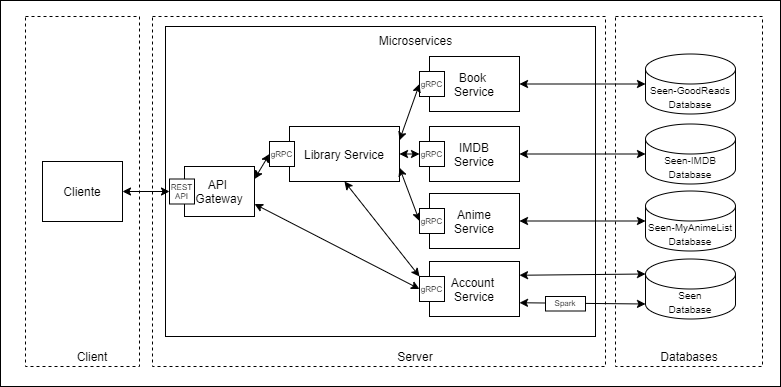
\includegraphics[width=\textwidth]{ CloudNativeAppArchitecture.png }
    \caption{Project's architecture.}
    \label{img:architecture}
  \end{figure}

  \subsection{Application}
    \subsubsection{Client}
    \fpar The Client should be able to access our API on his browser:
    \begin{center}
      \url{https://recommendations.sytes.net}
    \end{center}
    \par The Swagger provides a user interface to use and test our calls by adding "/ui" to the end of the url above.

    \subsubsection{Server}
    \fpar In total there are 7 different microservices working at the same time. Every single one of them runs on Google Cloud, inside the same cluster but in different dockers.
    \par Our reasoning was to have an entrance microservice, which would redirect the request to the microservice responsible for that type of request, for example when sending a request for a page in our library, the API Gateway receives that request and sends it to the Library Service, which is responsible for asking for books, movies and animes to the Book, IMDB and Anime Services, respectively, and then put them together in just one response, which is then sent to the API Gateway, to be shown to the Client.
    \par This API Gateway service also has the responsibility of transforming the REST requests from the Client to gRPC requests that are used internally, between Services.
    \par From the total of 7 microservices, 5 are responsible for the database connection, meaning that they are responsible for translating the request they receive into inserts, updates, removes or queries to the database. They are also responsible for translating responses from the database into responses that can be understood by the other microservices.

    \subsubsection{Databases}
    \fpar Every database has a service that has the responsibility to access and manage it. While 3 of the databases are hosted by \href{https://www.mongodb.com/}{MongoDB}, a NoSQL database, the last one is an SQL database hosted on an external server. This last database was initially hosted on Google Cloud, however we removed it from there, because it was costing us a lot of money.
    \par For the Books', Movies' and Animes' databases, we used a NoSQL database since we might have had to change the format of our documents, meaning that if we had an SQL database we would need to drop the entire database and repopulate it again every time we decided to change the schema. MongoDB provides a very easy and intuitive python implementation to work with, which was also a factor to consider when selecting the type of databases that we would be using.
    \par However, for the Users' database we used an SQL one, because we already knew what we wanted from the User and we knew we would use structured data for it.

    \subsubsection{Spark}
    \fpar For a posterior addition like it was with Spark we created a new microservice, this microservice would be responsible for both the Spark request we provide, this service receives the gRPC requests from the API Gateway and then processes them, creating job to send to the Google Cloud where we have a Cluster with the sole purpose of running these types of jobs.

  \subsection{Technical}
    \subsubsection{Client}
    \fpar TODO

    \subsubsection{Server (Microservices)}
    % falar do istio
    \fpar TODO

    \subsubsection{Databases}
    \fpar TODO

    \subsubsection{Spark}
    \fpar TODO

\section{Implementation}
\label{sec:implementation}
\fpar We actually made 2 different implementations, because before deploying it to the cloud, where we would pay for using the service, we made a local version, that would work locally, by running a script, it's very similar to the cloud implementation, but still has its quirks that are not crucial for the cloud deployment.

    \subsection{Client}
    % TODO

    \subsection{Server (Microservices)}
    % falar do dns resolver, usado localmente e não 
      \subsubsection{Docker Compose}
      \fpar For the micro-services deployment we use a docker-compose file, which defines each microservice.
      \par We give them a name, a build stating that we are using a Dockerfile and where the context of this microservice is (its folder, with its required content).
      \par For the image, hostname and container name we use the same name as the docker-compose microservice name we just gave.
      \par At last, we pick which ports we want to use for each microservice, they are crucial for the project to behave properly.
      \par We do the steps stated before for every single microservice inside the docker-compose, but we still have changes to do, since the API Gateway services sends request to the Spark Connector, Account and Library, we add them as environment variables, meaning when running the python file we can fetch the generated IP and then use it to connect with gRPC channels. For the library we add all the services responsible for the databases, which are the Services Book, Imdb, Anime and Account.

      \subsubsection{Dockers}
      \fpar With the microservices to create a docker image we used dockerfiles, they are really simple, they basically have everything they need in the folder they are in, and just make a new folder called service, and copy the current folder inside the newly created one.
      \par After copying we run the installation of the requirements, using pip and the "requirements.txt" file.
      \par Then the same port, used on the docker-compose file before, it's exposed to be accessible from outside this controller ambient/sandbox.
      \par Finally, we define the entry point as the python file containing all the business of this microservice.

      \subsubsection{Proto Files}
      \fpar % TODO

    \subsection{Databases}
    % TODO

    \subsection{Spark}
    % TODO


\section{Evaluation and validation}
\label{sec:evaluation_and_validation}

    \subsection{Evaluation}
    \label{sec:evaluation}

    \subsection{Validation}
    \label{sec:validation}

\section{Cost analysis}
\label{sec:cost}

\section{Discussion}
\label{sec:discussion}
    \subsection{Results}
    \label{sec:results}

    \subsection{Analysis}
    \label{sec:analysis}

\section{Conclusions}
\label{sec:conclusion}

    \subsection{Contributions}
    \label{sec:contributions}

      \subsubsection{51034 - Tiago Carvalho}
      \subsubsection{51058 - Diogo Lopes}
      \subsubsection{51072 - Miguel Saldanha}
      \subsubsection{51080 - João Roque}
      \subsubsection{51111 - João Afonso}

    \subsection{Future alterations}
    \label{sec:alterations}

\end{document}